%% Template para dissertacao/tese na classe UFBAthesis
%% versao 1.0
%% (c) 2005 Paulo G. S. Fonseca
%% (c) 2012 Antonio Terceiro
%% (c) 2014 Christina von Flach
%% www.dcc.ufba.br/~flach/ufbathesis

%% Carrega a classe ufbathesis
%% Opcoes: * Idiomas
%%           pt   - portugues (padrao)
%%           en   - ingles
%%         * Tipo do Texto
%%           bsc  - para monografias de graduacao
%%           msc  - para dissertacoes de mestrado (padrao)
%%           qual - exame de qualificacao de mestrado
%%           prop - exame de qualificacao de doutorado
%%           phd  - para teses de doutorado
%%         * Media
%%           scr  - para versao eletronica (PDF) / consulte o guia do usuario
%%         * Estilo
%%           classic - estilo original a la TAOCP (deprecated) - apesar de deprecated, manter esse.
%%           std     - novo estilo a la CUP (padrao)
%%         * Paginacao
%%           oneside - para impressao em face unica
%%           twoside - para impressao em frente e verso (padrao)

% Aten��o: Manter 'classic' na declaracao abaixo:
\documentclass[en, msc, classic, a4paper]{ufbathesis}

%% Preambulo:

\usepackage[utf8]{inputenc}
\usepackage{graphicx}
\usepackage{lipsum}
\usepackage{hyphenat}
\usepackage[usenames, dvipsnames, table]{xcolor}
\usepackage{booktabs}
\usepackage{pifont}
\usepackage{multirow}
\usepackage{listings} 
\usepackage{colortbl}
\usepackage{xfrac}
\usepackage[FIGTOPCAP]{subfigure}
\usepackage{subfig}
\usepackage{float}
\graphicspath{ {images/} }

% Universidade
\university{Universidade Federal da Bahia}

% Endereco (cidade)
\address{Salvador}

% Instituto ou Centro Academico
\institute{Instituto de Matem\'{a}tica}

% Nome da biblioteca - usado na ficha catalografica
\library{Biblioteca Reitor Mac\^{e}do Costa}

% Programa de pos-graduacao
\program{Programa de P\'{o}s-Gradua\c{c}\~{a}o em Ci\^{e}ncia da Computa\c{c}\~{a}o}

% Area de titulacao
\majorfield{Ci\^{e}ncia da Computa\c{c}\~{a}o}

% Titulo da dissertacao
\title{A variability based model to generate and disseminate emergency public communications}

% Data da defesa
% e.g. \date{19 de fevereiro de 2013}
\date{20 de Julho de 2018}
% e.g. \defenseyear{2013}
\defenseyear{2018}

% Autor
% e.g. \author{Jose da Silva}
\author{Jorge Fernando Silva Pereira Filho}

% Orientador(a)
% Opcao: [f] - para orientador do sexo feminino
% e.g. \adviser[f]{Profa. Dra. Maria Santos}
\adviser{Manoel Gomes de Mendonça Neto}

% Orientador(a)
% Opcao: [f] - para orientador do sexo feminino
% e.g. \coadviser{Prof. Dr. Pedro Pedreira}
% Comente se nao ha co-orientador
\coadviser{Renato Lima Novais}

%% Inicio do documento
\begin{document}

%% Parte pre-textual
\frontmatter

\pgcomppresentationpage




%%%%%%%%%%%%%%%%%%%
% Resumo em Ingles
%%%%%%%%%%%%%%%%%%%

\abstract

% A crisis is unpredictable by nature. Despite this, it presents patterns that can help communicators to anticipate problems to give faster and better responses to emergency situations. The current solutions for emergency public communication focus on the dissemination of a single message through different communication channels, for all audiences. This strategy is against the good communication studies because different audiences will receive information that is not of interest to them or that will not be presented in the best way for their understanding (e.g, technical and statistical information for the lay public). An inappropriate public communication message can amplify the perception of risk from at the public,and thus, be adding to the insecurity and lead to the creation of noises in communication that are difficult to fix in the progress of the crisis. Several studies have been conducted to propose good communication principles, among which we can highlight: be first (for the public the first source is the most reliable); be right (accuracy establishes credibility); be credible (honesty and truthfulness are essential during a crisis); communicate repeatedly (whenever possible, keep the public informed); and communicate by different tools, media and communication channels (never rely on a single method of communication). Our research, considers these principles to propose a computational model for public communication of emergencies. We mapped the variability in the process of communication of emergencies in order to ensure flexibility of configuration in different scenarios and types of emergencies. The main contribution of our research is a variability based approach to support customised communication of the emergencies and its consequences targeted to proper audiences. In this approach, we defined four variability behaviours in the content of the sentences in order to support the adaption according to the emergency state information. This research is being developed inside of a larger research project named RESCUER\footnote{Rescuer Project - http://www.rescuer-project.org} -- a joint Brazil-Europe initiative, involving nine research and industry organisations in four countries (Brazil, Austria, Germany and Spain). RESCUER aims at developing an interoperable solution to support command centres in quickly managing emergencies, based on reliable and intelligent analysis of crowdsourcing information mashed up with open data.
%The term “crisis communication” is usually used in two ways: (1) to refer to communication between organisations involved in managing the crisis and (2) to refer to communication from the emergency management to inform and alert the public about the emergency. The latter definition fits best the scope of our work, as it focuses on minimising the challenges faced by communicators while informing and alerting the public about an emergency. 


A crisis is unpredictable by nature, but it presents patterns that can help communicators to anticipate problems and give better responses to emergency situations. Current solutions for emergency public communication focus on the dissemination of a single message through different communication channels. This strategy goes against good communication practices because different audiences have different information needs. Inappropriate public communication messages create noise and can amplify the perception of risk and insecurity.  Our research proposes a computational model for public communication in emergencies. It maps and models variability in emergency communication processes to ensure the flexibility and adaptability of the communication configuration for different emergency scenarios. The model aims to facilitate the rapid construction of customised and consistent emergency communications, over different channels, for different audiences. The model was developed as part of a larger research project named RESCUER, which uses crowdsourcing information to monitor and manage emergency situations. To evaluate the communication model, a proof of concept, named RESCUER News, was built and evaluated in simulations involving real public and operational forces, over three distinct emergency scenarios. 




 %As proof-of-concept we developed a solution for public communication called “RESCUER News”. The solution was then used by experts on emergency management of two countries (Brazil and Austria), tested in simulations of emergencies in two different scenarios (Industrial Parks and Large Scale Events).
\begin{keywords}
Emergency Public Communication; Crisis Communication; Document Variability; 
\end{keywords}



%%%%%%%%%%%%%%%%%%%
% Sumario / Indice
%%%%%%%%%%%%%%%%%%%

% Comente para ocultar
\tableofcontents

% Lista de figuras
% Comente para ocultar
\listoffigures

% Lista de tabelas
% Comente para ocultar
\listoftables

%% Parte textual
\mainmatter

% Eh aconselhavel criar cada capitulo em um arquivo separado, digamos
% "capitulo1.tex", "capitulo2.tex", ... "capituloN.tex" e depois
% inclui-los com:
% \include{capitulo1}
% \include{capitulo2}
% ...
% \include{capituloN}
%
% Importante: 
% Use \xchapter{}{} ao inves de \chapter{}; se n�o quiser colocar texto antes do inicio do capitulo, use \xchapter{texto}{}.


\xchapter{Introduction}{}\section{Context} 
% \label{chapter:introduction}
%

Crisis and emergency are ``sudden and usually unforeseen event that calls for immediate measures to minimise its adverse consequences" \cite{dha1992internationally}. Basically, the term ``crisis communication" is used in two ways: when we refer to communication between organisations involved in managing the crisis and when we refer to necessity of the emergency management to inform and alert the public about the emergency \cite{cdc2014}. The latter definition fits best the scope of our research, being developed considering to minimise the challenges faced by communicators while performing this task. 

Establish an effective communication with the public during a crisis is a key measure for the crisis mitigation. A set of studies \cite{tinker2010}\cite{cdc2014}\cite{glik2007}\cite{seeger2006best} says that is essential maintaining the public informed about the occurrence of an emergency and its consequences. Among the benefits of this action, we can highlight: reduce crisis-related uncertainty; correct misunderstandings, rumours, or unclear facts; and reduce emotional turmoil and anxiety from the public. In addiction, this studies propose good communication principles among which we can highlight some basic principles: be first (for the public the first source is the most reliable); be right (accuracy establishes credibility); be credible (honesty and truthfulness are essential during an crisis); communicate repeatedly (whenever possible, keep the public informed); and communicate by different tools, media and communication channels (never trust on a single method of communication).

%The present solutions for public communication were designed to disseminate a message to many publics. It is an ineffective approach, whereas it the great challenge for the public communication team is creating, quickly, appropriate messages according to the information needs of each public audience during a turbulent moment, like is an emergency.

%Basically, the term ``crisis communication" is used in two ways: when we refer to communication between organisations involved in managing the crisis and when we refer to necessity of the emergency management to inform and alert the public about the emergency \cite{cdc2014}. The latter definition fits best the scope of our research, being developed considering to minimise the challenges faced by communicators while performing this task.

%Several studies have been conducted to propose good communication principles \cite{tinker2010}\cite{cdc2014}\cite{glik2007}, among which we can highlight some basic principles: be first (for the public the first source is the most reliable); be right (accuracy establishes credibility); be credible (honesty and truthfulness are essential during an crisis); communicate repeatedly (whenever possible, keep the public informed); and communicate by different tools, media and communication channels (never trust on a single method of communication).

%Our research, considers all concepts, principles and best practices described previously to propose a  computational model for public communication of emergencies. We mapped the variability in the processor of communications of emergency in order to ensure flexibility of configuration in the different emergency scenarios and/or type of emergencies. Furthermore, we use our variability analysis to design our approach to support customised communication of the emergencies and its consequences targeted to a proper audience. In this approach, we define four variability's behaviour in the content of the sentences according to the emergency state information. Finally, as proof-of-concept we develop a solution for public communication called "RESCUER News". RESCUER News was used during our research by experts of emergency management of two countries (Brazil and Austria), in simulations of emergency occurred in two different scenarios (Industrial Parks and Large Scale Events).

%This research is being developed inside of a larger research project named RESCUER\footnote{Rescuer Project - http://www.rescuer-project.org} -- a joint Brazil-Europe initiative, involving nine research and industry organisations in four countries (Brazil, Austria, Germany and Spain). RESCUER aims at developing an interoperable solution to support command centres in quickly managing emergencies, based on reliable and intelligent analysis of crowdsourcing information mashed up with open data.

\section{Motivation}

In the early hours of December 3, 1984, in the city of Bhopal, India, occurred the biggest chemical disaster for the present day \cite{broughton2005bhopal}. During this incident, 40 tons of toxic products were released into the atmosphere. More than 500 thousand people were exposed to toxic substances, causing 3 thousand direct deaths and 10 thousand due to diseases caused by the inhalation of gases. During the emergency, the managers of the affected factory initially denied the occurrence of emergencies, subsequently claimed to be victims of a terrorist act. Post-tragedy investigations indicated that the real cause was the lack of maintenance and lack of effective security measures as the main causes of the disaster. 

The consequences of these disasters have been amplified due to wrong communication practices. The omission of information from the crisis managers made the medical aid shortfall since the doctors did not know the cause of the intoxication of the hundreds of people who arrived at the hospitals. In addition, measures to protect the population, such as evacuation of communities that would be affected by the toxic cloud in a timely manner, could not be carried out due to a lack of information on the emergencies that were in course.

The disaster that took place in 2016 in the municipality of Mariana in Brazil, caused by the rupture of the retention dam of mining tailings is a recent example of disaster with serious failings in public communication of emergencies. This disaster affected the population of more than 5 districts without any warning from the managers. The tragedy was marked by communication failures to the affected population which caused the death of 19 people dragged through the mud \cite{escobar2015mud}.


During crisis and emergency situations, establish a good communication between the emergency management team and the general public is a key step to minimise the impact on the affected public. However, the process to establish a good communication is not an easy task. Crisis and emergency are complex situations involving stress, panic, fear and uncertainty \cite{reynolds2007crisis} both to the communication team and the people affected directly and indirectly by the consequence of the crisis.

In addiction, the communicators need to ensure that the appropriate messages will be sent to each target audience according to their interests\cite{panamericanhealthorganization2009}. This includes write the messages using appropriate vocabulary, provide you only the most relevant information, ensure the consistency of each message and your trustworthiness. 


Those limitations motivate us to do more detailed research about the process of communication of crisis and emergencies to the public and propose an integrated model in order to help the public communication team write and disseminate appropriated messages according to the interest of each target audience with a reduced effort.

\section{Research Problem}

The current solution for public communication during crisis and emergency situations were designed to disseminating one message to all affected public. In general, those solutions are focused almost totally entirely on the task of disseminating a public communication for several communications channels. The dissemination of messages to the affected public by several communications channel is an important step in the public communications of crisis and emergencies, on the other hand, does not make sense disseminate public communication messages by various communication channels if this message does not meet the information needs of each different target audiences. This is the main problem with this strategy, the dissemination of information that is not in accordance with the information needs of the specific audiences could create an "information overload" in a situation that the public is incapable of juggling multiple facts\cite{cdc2014}. 

Many studies and guides to good practice have been proposed over the last few decades with a view to reducing emergency and service impacts. The problem on the creation and dissemination of public communication during crisis and emergency situations may be explained by the complexity and risk of life's involved on this situations. The need to inform affected people as quickly than possible and ensuring the consistence of the information in a situation that have ``more questions than answers \cite{cdc2014}" is a grant challenger to the emergency communicator.

The solutions proposed for public communication during emergencies focus almost exclusively on the task of disseminating a single message through the most diverse means of communication. The dissemination of information through multiple communication channels is considered a good practice of public communication, but it is not the only challenge for the public communication team. Effective communication with the public during emergencies will, in a simplified way, reliably obtain reliable information, formulate consistent messages and respond to the interests of each public, and finally disseminate them through various communication channels in order to achieve The most amount of stakeholders quickly.

\section{Research Question and Goals}

%The objectives of this research are: 1) to identify public communication challenges coming up in an emergency; 2) to elicit existing users and contextual information needs in an emergency; 3) to define the relevant information adaptation according to different target audiences and phases of an emergency; and 4) to implement this context-aware approach in our RESCUER News systems. The novelty is to support (semi-)automatic customized communication of the incident targeted to different audiences. 

The research question that guides this master thesis is \textbf{“How to reduce the effort of public communication team to transmit relevant and consistent information, according to the interest of each target audience, during the course of an emergency?”}.

The general objective of this dissertation is to present a model for public communication during crisis / emergency situations. To this end, will be made an approach to public communication, elaborated seeking to cover the whole process of communicating of an emergency, that is, obtaining information from reliable sources, making appropriate communications to each target audience and finally, the dissemination of public communications by several communication channels.

To this end, we conceived a model based on the results of our analysis of the variability of the different factors that influence the communication in an emergency; seeking behavioural patterns in the variation of contents of the reports according to the current information of the emergency, the type of incident, the target public, and type of communication (short or extended); variations in the configuration according to the emergency scenario; and in the format of the message according to the different communication channels.

As specific objectives can be cited:

 \begin{itemize}
   \item Make a study of the good practices of emergency communication, especially those that are related to the content that will be transmitted;
   \item Present a new approach to creating documents from dynamic models with behaviours that adapt to the current state of the emergency;
   \item Implementation of a solution for emergency communication based on the proposed model;
   \item Conducting an evaluation with specialists in public communication in real emergency situations to measure quality in use and product in order to validate our proposal.
 \end{itemize}

%\section{Scope Limitation}

\section{Research Benefits}


A contribution from this master thesis is the proposal of a computational model to assist public communicators in the task of creating and disseminating communications during emergency situations. We proposed this model from the survey of the good practices present manuals of good practices in public communication of emergencies and by the practical experience of our partners specialise in the management of the crisis in the industrial park and large scale events.  

Our research also contributes with a study of the variability present in the process of public communication of emergencies, mapping the commonalities in the different aspects relevant to the configuration of an solution for public communication of emergencies or that affect (directly or indirectly) the content of the public communications releases.

An important contribution of our work is our novel approach to generate texts from dynamic models who adapt to the current state of the emergency, in other words, contents can be included or removed automatically according to the type of incident and/or type of Incident that is communicating, for example. In addition, we present four behaviours for varying the content of the sentences of the public communications according to the current status of the emergency.

Finally, another contribution of our work is our emergency communication solution called RESCUER News. We are developing the Rescuer News as a proof-of-concept of our proposed model.

\section{Methodology}

Figure \ref{fig:methodology} presents the methodology, with its phases and activities, considered to achieve the goals of this study.


\begin{figure}[ht!]
\begin{center}
  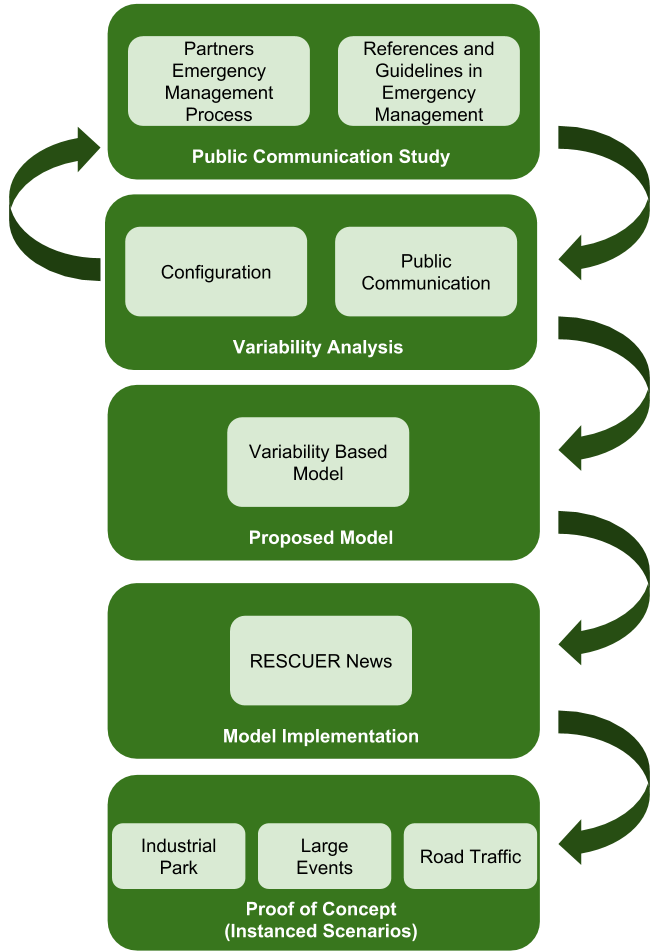
\includegraphics[width=0.50\linewidth, keepaspectratio]{images/Methodology.png}
\caption{Overview of the Research Methodology}
\label{fig:methodology}
\end{center}
\end{figure}


Our research starts with the identification of about how the public communication occurs in real situations. We analysed the processes that our partners applied in these situations and, in parallel, we looked for guides to good practice and manuals for an effective emergency public communication.

After the collection of information, we performed the variability analysis inside of the emergency public communication life cycle.

Next, we developed a conceptual model that would allow configuration for the multiple possible scenarios of an emergency. Based on this model we have developed the RESCUER News, a functional prototype for public communication within ERTK Module of the RESCUER Project.

Finally, as proof of concept we set up our prototype for a series of demonstrations and evaluations within the RESCUER Project.

In the Chapters \ref{chapter:}

\section{Academic Results}

In this section, we present the academic achievements within the scope of this master's thesis.

\subsection{Publications}

During this master's thesis we write the following papers: 

\textbf{Published:}

\begin{itemize}
   \item \emph{Challenges in crowd communication for emergency management}, in Brazilian Congress of Software (CBSOFT), SCrowd 1st WORKSHOP ON CROWDSOURCINGSYSTEMS, 2015 \cite{pereirachallenges};
   
   \item and \emph{Rescuer News: A public communication tool for crisis situations}, Conference on Computer-Supported Cooperative Work and Social Computing (CSCW), Workshop  on  Collaboration  and  Decision  Making  in  Crisis  Situations(CADMICS), 2016 \cite{cscw2016}
  
   \item \emph{On the Design of a Contextual Emergency State Builder with Multiple Data Sources}, First IEEE Summer School on Smart Cities, 2017 \cite{pereiraetall2017}
  
\end{itemize}

\textbf{Submitted:}

\begin{itemize}
   \item \emph{A Variability Based Model to Generate and Disseminate Emergency Public Communications}, in Expert Systems with Applications: An International Journal, 2018 
\end{itemize}

\textbf{Accepted but not published (by authors' choice):}

\begin{itemize}
   \item \emph{Context-Aware Public Communication for Crisis Management}, in The Tenth International Conference on Software Engineering Advances (ICSEA) ,2015 (Short Paper)
\end{itemize}

\textbf{Submitted but not accepted for Publish:}

\begin{itemize}
   \item \emph{Context-Aware Public Communication for Crisis Management}, in ACM Symposium on Applied Computing, 2016 
\end{itemize}


\subsection{Participating in Research Projects}

As mentioned above, this research was developed inside of the Rescuer Project, more specifically, as part of the ERTK component. 

Among the activities developed in the project we can highlight: a study on public communication of emergencies including the organisation of 4 workshops with specialist in crisis communication; the publication of two articles in workshops focused on crisis and emergencies; organisation of simulation to evaluate the prototypes developed in the project; and the development of a solution for communication with the public during crisis and emergencies called ``Rescue NEWS". 


\subsection{Research Exchange}

Research Interchange was conducted during the 1 year period (October 2015 to November 2016) as a invited researcher at the Fraunhofer Institute for Experimental Software Engineering (IESE)\footnote{https://www.iese.fraunhofer.de/en.html}, in the city of Kaiserslautern, Germany. The IESE is one of the most widely recognized software engineering institutions world-wide and takes a lead in Europe. Among your competences, we can highlight: Requirements Engineering,  Software Architecture, Safety Engineering and User Experience.

During the period in the institute, the student worked on tasks related to his master's research and on tasks related to performing demonstrations and evaluations of the components of the RESCUER Project.

\section{Document structure}

The remainder of this text is structured as follows: Chapter \ref{cap:2} presents the main concept of emergency public communication, the related work in document variability and an analysis of the present solution for public communication

Chapter \ref{cap:3} we present our mapping of variability in the process of public communication of emergencies, the conceptual model proposed in this research, the academic results and our activity schedule from the rest of this master thesis.

%\include{sections/theoreticalBasis}
\xchapter{Background}{} \label{chapter:background}

In this section, we briefly introduce main concepts relevant to understand the developed work. 

\section{Public Communication of Emergencies} Emergencies are defined as critical situations caused by incidents, natural or man-made, that require measures to be taken immediately to reduce their adverse consequences to life and property \cite{dha1992internationally}. The adverse and therefore undesired consequences of an emergency give rise to a crisis.
An emergency comprises a random and totally unexpected event. However, it presents patterns that can help communicators anticipate problems and be able to give an immediate response \cite{cdc2014}, hopefully avoiding a crisis.

However, emergency and crisis are used as synonym in the field of public communication. In this context, the term "crisis communication" is used with two meanings. The first one refers to the communication among organisations involved in the emergency management. The second one is related to the need of the emergency management to inform/alert the public about the emergency \cite{cdc2014}. The last definition is the one that best fits the scope of our research.

This chapter describes the main characteristics of public communication in emergencies/crises. Additionally, it presents concepts and best practices on Crisis and Emergency Risk Communication.

\subsection{Crisis and Emergency Risk Communication}

One key aspect of emergency management is communication, which can help people and organisations to handle the emergency situation in a better way. The challenge of this activity is to establish a good strategy for communication with the partners that should be informed. A simple definition for Crisis and Emergency Risk Communication (CERC) is: a set of principles that aim to guide emergency managers to know what to say, when to say, how to tell and thus preserve or win the public's confidence during a crisis \cite{cdc2014}.

After analysing a set of studies in this field, we selected the CERC study \cite{cdc2014} to provide detailed information on crisis and emergency communication. CERC is a general theoretical framework developed by Centres for Disease Control and Prevention (CDC) of the United States of America. Its basic principle of communication is: be first, be right, and be credible.
Two additional concepts are essential to understand the CERC principles: Crisis communication and Risk communication.

\begin{itemize}
   \item \textbf{Crisis Communication:} it refers to communication activities of an organisation that is facing a crisis. However, the term may be associated either with the management of emergency or the effort involved in the task of alerting and keeping the public informed about an incident \cite{cdc2014}. 
   \item \textbf{Risk Communication:} it comprises the “information exchange about health risks caused by environmental, industrial, or agricultural, processes, policies, or products among individuals, groups, and institutions” \cite{glik2007}.
 \end{itemize}

CERC arises from the application of risk communication principles in crisis communication, i.e., it incorporates communications about possible risk factors into the communication of the crisis evolution \cite{reynolds2005}.

\subsection{The CERC Lifecycle}  \label{cercPhase}
Despite a crisis being a random and totally unexpected event \cite{cdc2014}, it presents patterns that support communicators to anticipate problems and give immediate response. A crisis can be divided into the following phases: pre-crisis, initial, maintenance, resolution and evaluation \cite{cdc2014} \cite{reynolds2005}.
 
 
\textbf{\\Pre-crisis phase\\}
In this phase, the goal is educational and it aims at preparing the public to know how to behave in an emergency situation. In this phase, it is important to test the public communication systems, detecting potential problems and ensuring their full operation in real crisis situations.

\textbf{\\Initial phase\\}
In the initial phase, the priority is to inform the general public and the affected people about the occurrence of the incident \cite{reynolds2005}. This information must be passed quickly, but ensuring its reliability. More specifically, the message content in the initial phase should have the following attributes: be simple, credible, accurate, consistent, and delivered on time \cite{cdc2014}.

The purpose of communication is to ensure:

\begin{itemize}
   \item the empathy and reassurance of the public, reducing emotional turmoil;
   \item the understanding of the responsibilities of the organisations involved in the crisis;
   \item that the public knows where they can get more information.
 \end{itemize}
 
 In both application scenarios of our research, incidents at industrial parks and at large-scale events, this phase is associated to the period between the arrival of the first reports of an incident at the command and control centre and the arrival of work forces at the place of the incident. The emergency status at the end of this phase is \textbf{"Being Controlled"}, as called by the emergency coordinators from industrial parks and large-scale events in the workshops that we carried out.
 
\textbf{\\Initial phase\\}
 
 Communication in the maintenance phase seeks to ensure that the public:
 
 \begin{itemize}
   \item understands the risks involved in the incident and how to prevent them;
   \item is instructed about misunderstandings or rumours;
   \item receives guidance on protective actions that should be taken;
   \item is aware of actions taken by emergency managers and workforces to control the incident.
   
 \end{itemize}
 
 
 This phase covers the period between the moment in which the workforces at the incident place start handling the incident (e.g., fighting the fire), which corresponds to the emergency status \textbf{“Being Controlled”}, and the moment in which they finish handling the incident per se, but they still need to take protective measures, which corresponds to the emergency status \textbf{“Under Control"}.
 
  \textbf{\\Resolution phase\\}
  
  In the resolution phase it is important that the communicator continues to provide information to the public about the incident, presenting the measures that are being taken to overdue the damages caused by the incident. At the end of this phase the status of the emergency is \textbf{“Finished”}.
  
  
  \textbf{\\Evaluation phase\\}
  
  The last phase starts after the crisis is finished. At this stage it is important that crisis managers analyse how the communication occurred during the crisis and propose actions to improve the process. During this phase, the documentation that reports the crisis and the lessons learned is elaborated. This phase start after the end of the emergency and, for this reason, is outside the scope of our research. 
  
\subsection{Steps of Crisis Response}

\begin{figure}[htb]
\begin{center}
  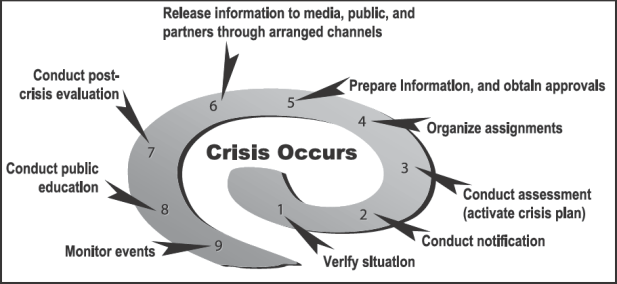
\includegraphics[scale=0.6]{images/CrisisSteps}
\caption{Steps of Crisis Response \cite{centers2006crisis}}
\label{fig:nineSteps}
\end{center}
\end{figure}

Usually, the initial moments of an emergency are considered the most chaotic. They are marked for the existence of uncertainty, panic and a great demand for information about the current situation, either for the emergency teams or for the external public affected directly or indirectly by its consequences. 

Faced with this critical situation, it is necessary that the crisis team promptly respond to the information needs of different publics. 

To help the crisis teams to effectively manage the most emergencies the CDC \cite{centers2006crisis} propose 9 generics communications steps to design a good crisis communication plan. The figure \ref{fig:nineSteps} shows each step proposed to crisis response.

\begin{enumerate}
   \item \textbf{Verify the Situation}: The first task for emergency response is the "situational awareness", i.e, get reliable information about the occurred facts from credible sources; 
   \item  \textbf{Conduct Notifications:} In the following, the crisis team needs to notify all partner (organisations and key people) involved in the crisis mitigation;
   \item  \textbf{Conduct Crisis Assessment:} The crisis team needs  to be continually updated about new information,  the severity of the situation, the target audience, and what information should be communicated;
   \item \textbf{Organise Assignments Quickly:} assign quickly, for your team and partners, of responsibilities, tasks and a consistent response to all communication needs; 
   \item \textbf{Prepare Information and Obtain Approvals:} Prepare Information and Obtain Approvals: is in this step, the crisis communication team will develop messages for public communication in a timely release;
   \item \textbf{Release Information through Prearranged Channels:} Select the target audience and the communication channels to disseminate rapidly the public communications. Prior to a crisis, is important that the crisis communication team identify the possible audience and the most appropriate communication channel for each;
   \item \textbf{Obtain Feedback and Conduct Crisis Evaluation:} Evaluate periodically the communication process during the crisis in order to detect possible communication problems. Feedback from key audience and media are a good way to make this evaluation;   
   \item \textbf{Conduct Public Education:} the period after the occurrence of a crisis is an opportunity to provide educational improvements on the population about the preparation for future crisis situations;   
   \item \textbf{Monitor Events:} Finally, is necessary observe the communication activities in social media, press, etc. to determine how to improve messages and the communication strategy. 
\end{enumerate}   

Some of these steps (Steps 2, 4, 8 and 9) are linked directly to the communication between organisations or people involved in the crisis management. This type of crisis communication is out of the scope of our research.

The step 7 and 9 relate to the monitoring and obtaining information from the repercussions generate by the crisis situation. This research is linked to the public communication of emergencies but is not related to the task of creation and disseminations of public communications.

The process to create and disseminate public communications can be described in 3 tasks: obtaining reliable information about the emergency, build appropriated messages for each target-audience and disseminate this messages, quickly, through multiple communication channels. These tasks are contained in the steps 1, 3, 5 and 6. The proposed computational model in this research was structured based on this steps.

 
  \subsection{Best Practices}
  
  Several studies have been conducted to propose good communication principles \cite{cdc2014} \cite{seeger2006best} \cite{goldfine2011best} \cite{glik2007} \cite{tinker2010} \cite{panamericanhealthorganization2009}.  Some of the principles are essential for effective communication with the public during an emergency:
  
  \begin{itemize}
   \item communicate repeatedly;
   \item be clear (use simple language and do not use technical terms, statistics or probabilities);
   \item communicate by different tools, media and communication channels (never trust on a single method of communication);
   \item transmit consistent information; and
   \item provide only relevant information.
   
 \end{itemize}
 
 The studies \cite{cdc2014} and \cite{cisvGuide} also indicate the basic information the crisis/emergency communicators need to know about an emergency situation:
 
 \begin{itemize}
   \item WHAT happened?
   \item WHERE did it happen?
   \item WHEN did it happen?
   \item WHO is involved?
   \item HOW did it happen?
   \item WHAT is currently being done?
      
 \end{itemize}
 
 About the content of the public messages, \cite{reynolds2007crisis} propose a set of good characteristics that those messages need to have. This principal is called “STARCC" and it maintains that the messages must be:
 
 \begin{itemize}
   \item Simple: Frightened people don’t want to hear big words
   \item Timely: Frightened people want information NOW
   \item Accurate: Frightened people won’t get nuances, so give it straight
   \item Relevant: Answer their questions and give action steps
   \item Credible: Empathy and openness are key to credibility
   \item Consistent: The slightest change in the message is upsetting and
dissected by all
      
 \end{itemize}

\section{Feature Modeling}

Software product line (SPL) \citep{malizia2010sema4a} is a software engineering method to abstract and represent the concept of variability in software that shares a set of similarities. Feature modelling is a compact visualization of different features of a SPL and its relationships. 

Feature modeling is one of the Feature-Oriented Domains Models presented by \cite{Kang1990}. Feature-Oriented Domain Analysis (FODA) is a domain analysis method proposed to support Software Reuse \citep{krueger1992software} at the functional and architectural levels. The main goal of this method is to manage the commonalities and variabilities within a product line.  

In the Feature Model, the features are arranged in a hierarchical structure. One feature (parent feature) can have sub-features (child features). 

The relationship between the parental feature and his sub-features can be of the type AND (all child must be selected); Alternative (only one sub-feature can be selected), or OR (one or more can be selected). 

The relationship between features is defined by two type of constraints: Implies and Excludes. When a feature needs one or more feature we have a relationship of Implies. When the opposite is true, the selection of one feature disables the selection of the other feature, we have the relationship of Excludes \citep{batory2005feature}.

We decided to model the variability of the emergency public communication domain do through feature modelling. We use this approach to guide the development of our variability based model in order to capable the addressing the different stakeholders’ needs in the most different scenarios of crisis/emergency.

\xchapter{Related Work and Present Solutions}{}\label{chapter:related} 
\textcolor{red}{Escrever introdução}
\section{Related Work in document variability}{}


The main contribution of our research is a variability based approach to support customised communication of the emergencies and its consequences targeted to proper audiences. Because of this, we explore the literature in order to identify related work in document variability.

There are proposals in the literature focusing exploring variability management techniques to build customised information for specific stakeholders. The information is usually represented by documents, as proposed by  \cite{penades2010}, which describes a process model for mass customisation of documents called Document Product Lines (DPL). Relying on SPL principles \citep{clements2002}, this work uses feature models \citep{Kang1990} to manage common and variable aspects of software development documents. The process model is realised by  DPLfw \citep{gomez2012dplfw}, a high-level design solution to support specialists on describing the variability of documents accordingly. DPLfw has been applied in several business domains to generate different DPLs (e.g. emergency plans \citep{gomez2012dplfw}, software manuals \citep{penades2012}, e-government \citep{penades2014},  customised recipes \citep{canos2013} and e-learning objects \citep{labib2015}). The DPLfw presents a complex process to specify and customise the document, this process is appropriated to large documents which demand large time intervals for your composition, not being proper to emergency public communication for not presenting such characteristics.

Karol et al. \citep{Karol2010} propose a tool for generating families of documents called Document Feature Mapper. This work also uses feature models to manage variability on families of documents. Each feature represents a fragment of the document (e.g. paragraphs, images) which varies as required. Despite the authors mapping the variability in several aspects, do not be considered the generating of documents in different formats, this is necessary for the dissemination of public communication using multiple communication channels. 

\cite{Rabiser2010} present an approach for automatic generation of product lines documents. They use the DOPLER \citep{rabiser2009} tool suite for modelling software artefacts and their respective variability and applies a Document Type Definition (DTD) called DOCBOOK \citep{walsh1999} for documents generation. Since this approach addresses the generation of product line documents, it cannot be applied to any other domain, such as public communication of emergencies.

%Limitações presentes em todos os papers
Public communication of emergencies requires the ability to build customised documents according to the audience in a quick way and deliver it considering all available communication infrastructures. The above mentioned proposals do not present solutions to cope with variability in communication network infrastructures. Furthermore, their tool support is limited, offering only plugins for the Eclipse\footnote{Eclipse - http://www.eclipse.org} Integrated Development Environment (IDE). Such an environment supports software development activities, it is not targeted to any other kinds of audience.

%como nosso trabalho atende às limitações dos outros artigos
Our proposal is designed to assist the public communication team. To do this, we design an assisted message edition of public communication models that vary, automatically, according to the emergency state. This allows the generation of specific messages according to the interest of each target groups from a unique public communication model.

\Section{Present solutions for public communication of emergencies} \label{chapter:PresentSolution}

There are several solutions for communication with civilians in case of an emergency. Some of them are used for public communication, while others are used for the guidance of the people involved in the emergency. 

In this section, we present some public communication solutions and highlight their main features. 
  

\subsection*{Twitter Alerts}

The social network Twitter\footnote{https://twitter.com} has developed a tool called “Twitter Alerts” \cite{twitteralerts}, whose goal is to provide authorities with a new way of disseminating information about an emergency. The Twitter alerts are disseminated with a specific visual identity via SMS and to twitter users. Figure \ref{fig:twitter} shows an example of Twitter Alerts. The image on the left shows the Twitter Alerts received by SMS and the image on the right shows a Twitter Alert received at the Twitter Mobile Application. To receive such notifications one must subscribe to the Twitter Alerts service.

\begin{figure}[]
\begin{center}
  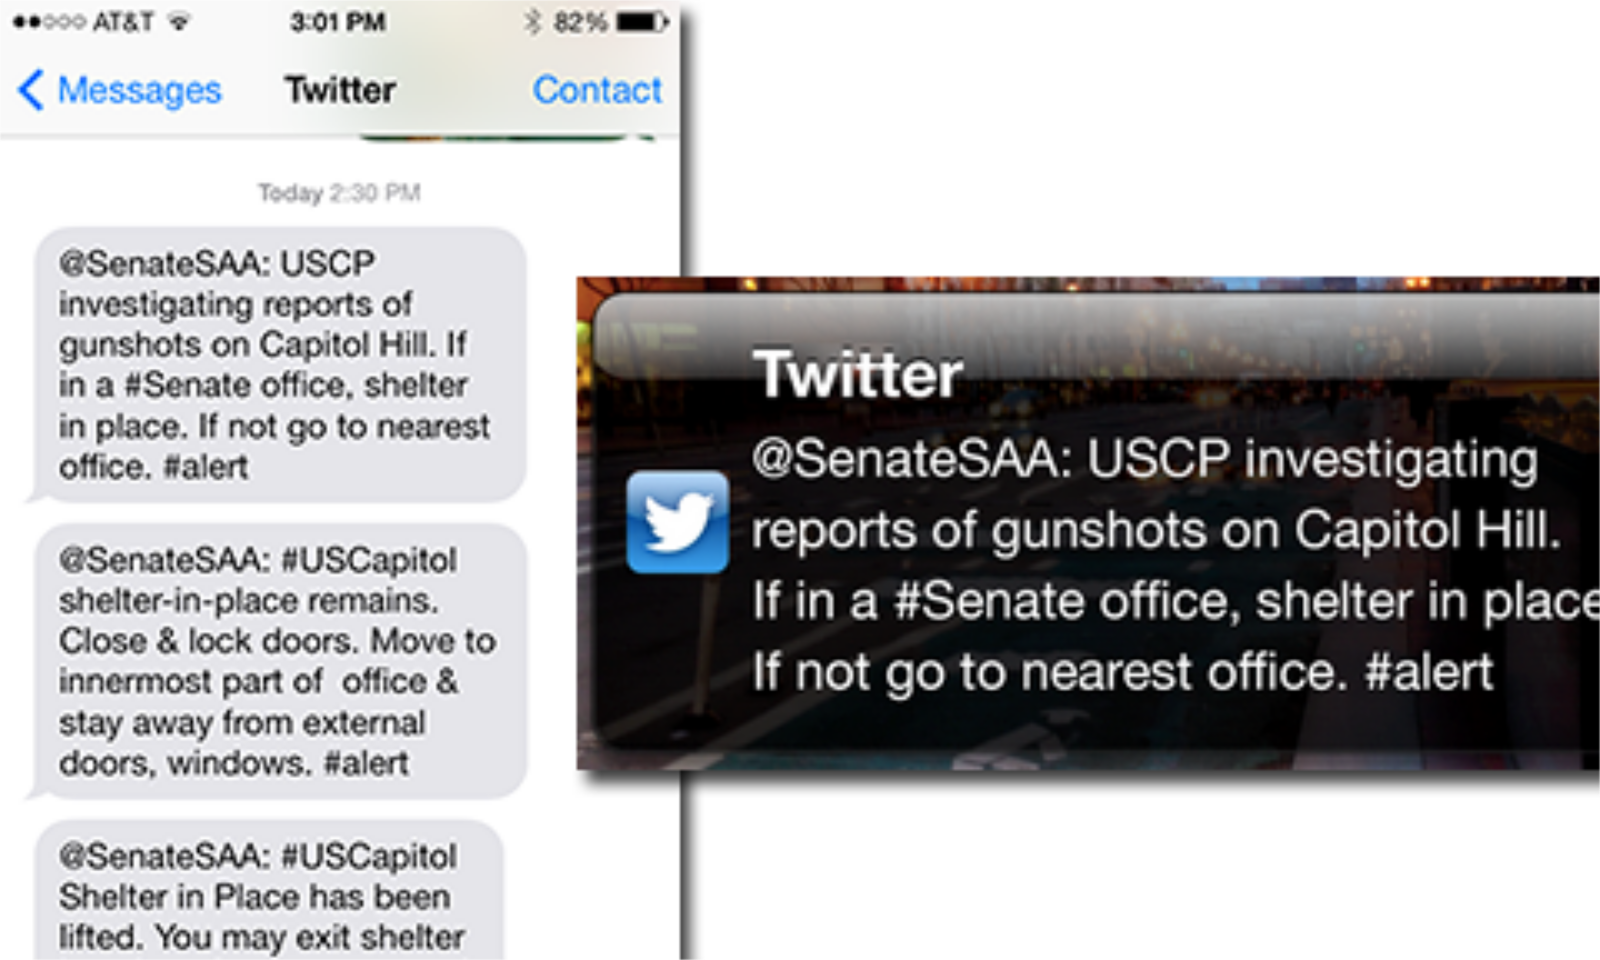
\includegraphics[width=0.7\linewidth, keepaspectratio]{twitterAlerts}
\caption{Example of Twitter Alerts messages. On the left an example of Twitter Alert Message notified by SMS and on the right by Twitter Mobile Application.}
\label{fig:twitter}
\end{center}
\end{figure}

\subsection*{Google Public Alerts}

Google Public Alerts is described as “a platform for disseminating relevant emergency alerts to users when and where they are searching for” \cite{googleAlerts}. The users are warned in two ways: a) by automatic emergency notifications sent through the mobile app Google Now (Android and IOS) and b) by customised search results when the user is looking for the situation of a specific emergency in the Google search engine. Figure \ref{fig:googleAlert} shows an example of search result (left side) and the emergency notification in Google Now (right side).

\begin{figure}[]
\begin{center}
  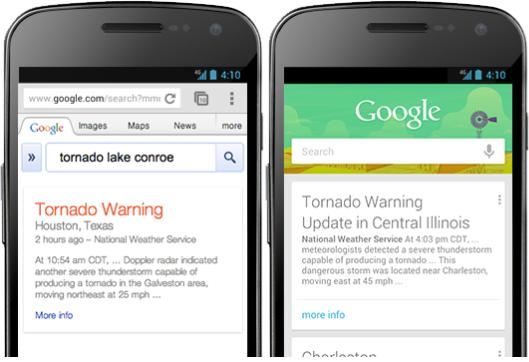
\includegraphics[width=0.7\linewidth, keepaspectratio]{googleAlerts}
\caption{Interface of Google Alert}
\label{fig:googleAlert}
\end{center}
\end{figure}

%\subsection*{Cell Broadcast Emergency Alerts}

%Cell Broadcast Emergency Alerts is a communication channel where messages can be issued to people in a specific area [13]. To receive emergency messages, the user’s mobile device must support the technology and the mobile telecommunication company must make the cell broadcast communication infrastructure available. Unlike SMS communication, solutions based on cell broadcast are free of network congestion, since such messages use an exclusive channel. Figure 3 shows an example of message received using this technology.

%\begin{figure}[htbp]
%\begin{center}
%  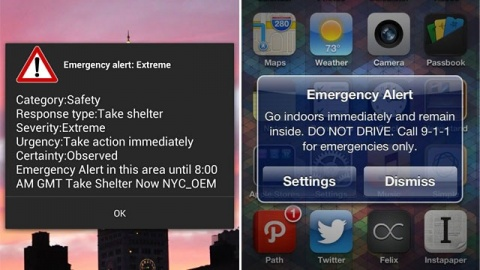
\includegraphics[height=5cm]{CellBroadcast}
%\caption{Examples of Cell Broadcast Emergency Alerts}
%\label{default-regular1}
%\end{center}
%\end{figure}

%There are governmental applications being developed for emergency communication using cell broadcast. For example, in the United States, the Commercial Mobile Alert System (CMAS) and the Wireless Emergency Alerts (WEA) [14], and, in the Netherlands, the NL-Alert [15]).

\subsection*{Israel National Message}

Developed by the Israeli government, the Israel National Message solution aims to “strengthen the spirit of the population and minimise subsequent damage in periods of war, national disasters and environmental emergency events by establishing a nationwide warning system that disseminates selective alerts and guidance messages to the population in real time, based on immediate control of all available and relevant channels in Israel” \cite{nationalMessage}. Figure \ref{fig:israelNM} presents the interface of the desktop solution.

\begin{figure}[]
\begin{center}
  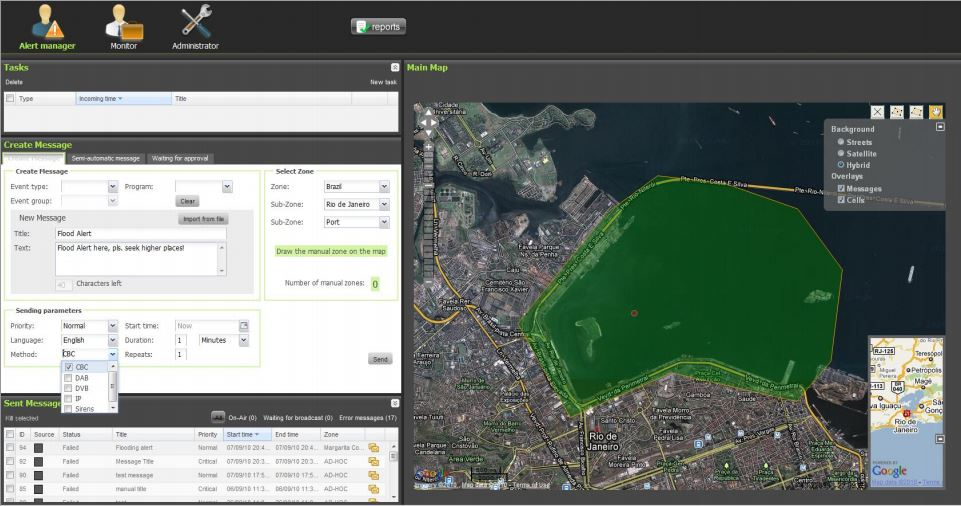
\includegraphics[width=0.85\linewidth, keepaspectratio]{israelNM}
\caption{Israel National Message (Personal Message Module)}
\label{fig:israelNM}
\end{center}
\end{figure}

This solution has a specific module for public communication called Personal Message, which allows the notification of an emergency occurrence to the population inside a specific area. This message can be sent by: cell broadcast, cell voice message, pager, TV, Radio, e-mail, website, Earthquake and Tsunami Warning service (ETWS) and sirens.

\subsection*{Alerts4All}
Alerts4All is a project developed in cooperation by 12 European partners. Its goal is to create “a complete communication framework for public alert” \cite{parraga2013complete}. This solution supports authorities during the preparation of emergency messages (Figure \ref{fig:allert4All}) and provides a specific communication protocol to transmit such messages. Therefore, it is necessary that TV, cell voice message, SMS, radio, GPS Navigator and sirens manufacturers implement the communication protocol created in the project. Figure \ref{fig:alert4allAlert} presents a practical example of alert message on TV.

\begin{figure}[]
\begin{center}
  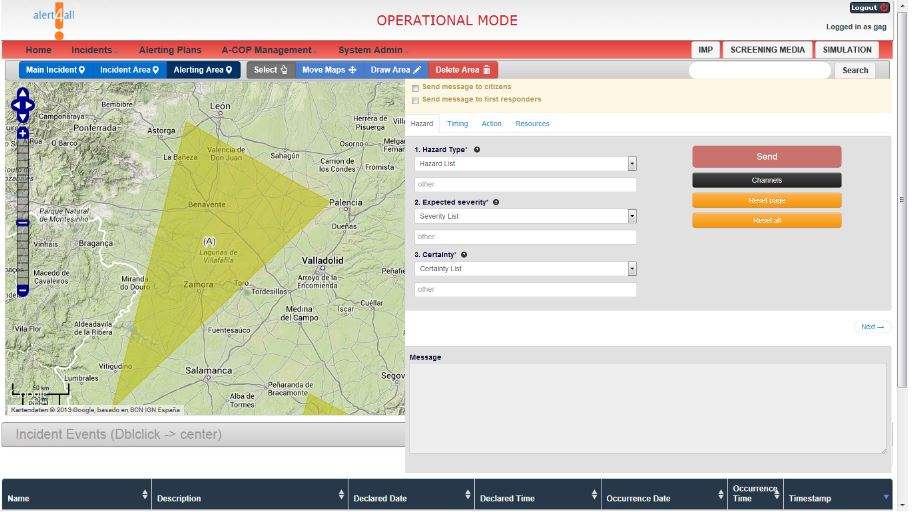
\includegraphics[width=0.8\linewidth, keepaspectratio]{alert4all}
\caption{Graphical user interface (GUI) of ALERT4ALL}
\label{fig:allert4All}
\end{center}
\end{figure}

\begin{figure}[]
\begin{center}
  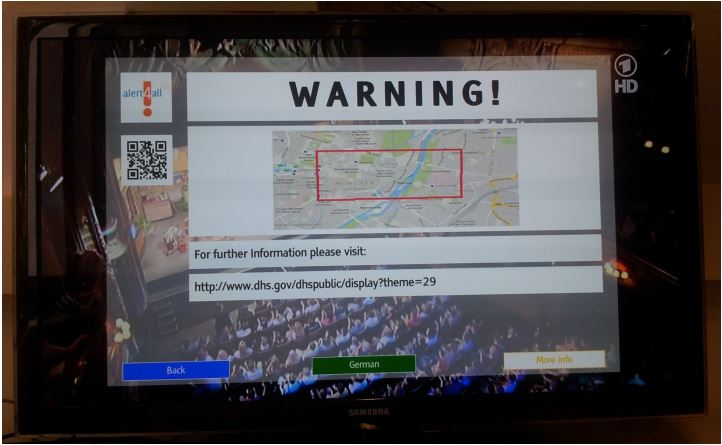
\includegraphics[width=0.8\linewidth, keepaspectratio]{alert4allAlert}
\caption{ALERT4ALL Alert Message on TV}
\label{fig:alert4allAlert}
\end{center}
\end{figure}

\subsection*{Code Red}

\begin{figure}[]
\begin{center}
  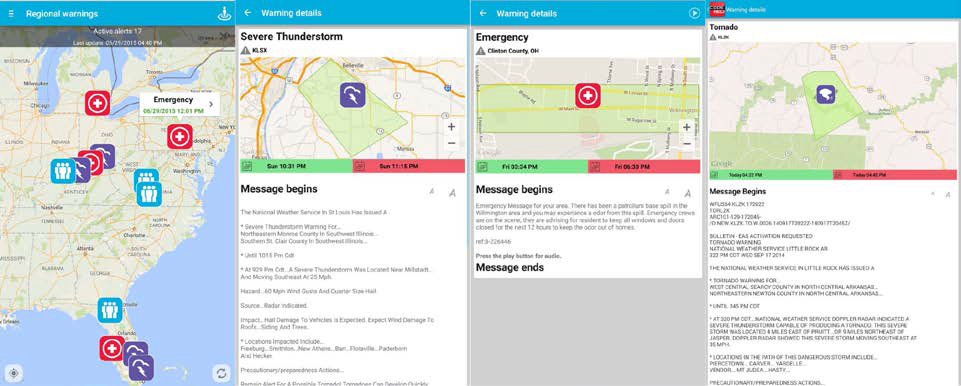
\includegraphics[width=0.8\linewidth, keepaspectratio]{codeRed}
\caption{Application screens of CodeRED Mobile Alert}
\label{fig:codRed}
\end{center}
\end{figure}

CodeRED (Figure \ref{fig:codRed}) is a solution developed by a company named Emergency Communication Network (ECN)\footnote{https://ecnetwork.com/} to support companies and authorities in reaching their audience during crisis and emergency situations. The audience can be notified by phone call, text message, e-mail, social media and CodeRED Mobile Alert application. Furthermore, the CodeRED is integrated with the Federal Emergency Management Agency (FEMA)\footnote{https://www.fema.gov/} of United States (U.S) and therefore allows sending alerts by WEA (Wireless Emergency Alerts)\footnote{https://www.fcc.gov/consumers/guides/wireless-emergency-alerts-wea}.

The emergency communicators can send messages using the web interface or by the mobile application called ACN Launcher (Figure \ref{fig:ecnLauncher}). CodeRED is in use by companies and public organisations in the United States and Canada.

\begin{figure}[]
\begin{center}
  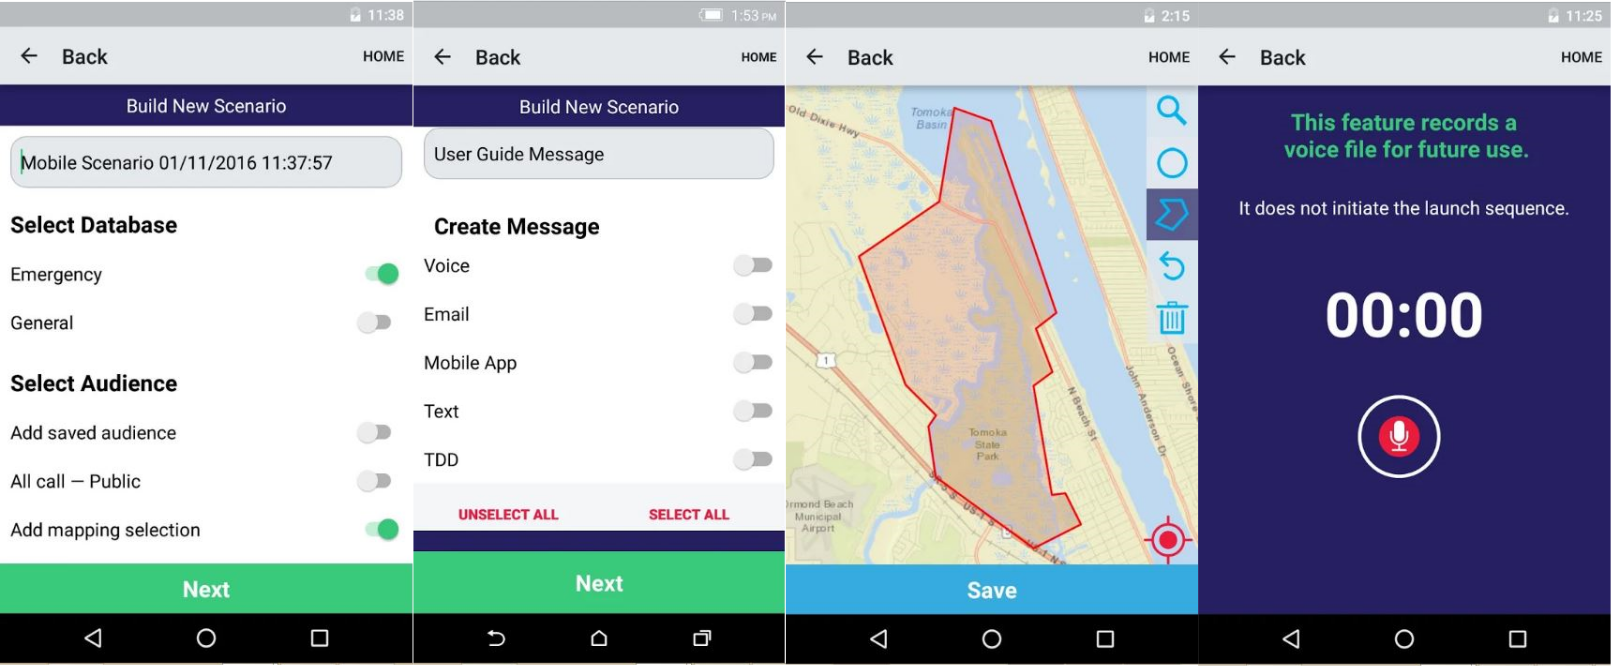
\includegraphics[width=0.6\linewidth, keepaspectratio]{ecnLauncher}
\caption{Application screens of ACN Launcher}
\label{fig:ecnLauncher}
\end{center}
\end{figure}

\subsection*{Crisis Communication Center}

\begin{figure}[]
\begin{center}
  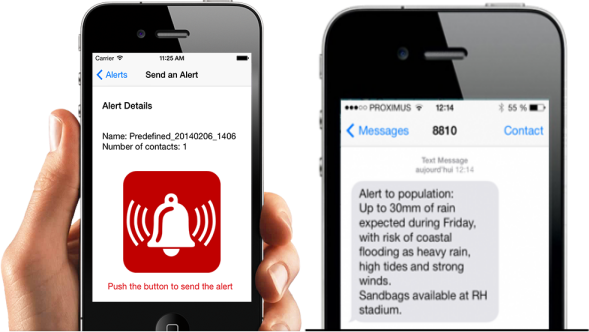
\includegraphics[width=0.6\linewidth, keepaspectratio]{crisisCC}
\caption{Application screens of Crisis Communication Center}
\label{fig:crisisCC}
\end{center}
\end{figure}

Crisis Communication Center is a crisis communication tool developed by the Belgian company “The Ring Ring”\footnote{http://www.ringring.be/}. The tool is a web-based solution that provides as main features the possibility of sending alerts by SMS, voice and e-mail. In addition, the tool allows the definition of message templates and includes the possibility of sending messages using a mobile application (Figure \ref{fig:crisisCC}).



\subsection{Limitations of the Existing Solutions}





Table \ref{comparisonTab} presents a comparison among the features present in the existing solutions. The following aspects were considered: assistance on the creation of messages (semi-automatic messages), sending of messages to specific areas (georeferenced) and the possibility of customisation of messages to specific groups of stakeholders. 

The aforementioned solutions are effective in disseminating reliable information about the emergency. However, the process of public communication of crisis/emergencies cannot be summarised to the sending of communications. Keeping the flow of reliable information to the communicator and helping him in the task of creating messages is crucial to ensure that this activity will be performed in an effective and efficient manner. 

In addition, the aforementioned solutions are not designed to create different messages for different target groups (e.g., press, public authorities or civilians). This is considered communication failures. This statement is based on the premise that “in a crisis, people don’t want to ‘just pick one’ of many messages, they want the best one or the right one to follow” \cite{reynolds2007crisis}.


% Please add the following required packages to your document preamble:
% \usepackage{booktabs}
% \usepackage[table,xcdraw]{xcolor}
% If you use beamer only pass "xcolor=table" option, i.e. \documentclass[xcolor=table]{beamer}
% Please add the following required packages to your document preamble:
% \usepackage{booktabs}
% \usepackage[table,xcdraw]{xcolor}
% If you use beamer only pass "xcolor=table" option, i.e. \documentclass[xcolor=table]{beamer}
\begin{table}[]
\centering
\caption{Comparison of Existing Solutions}
\label{comparisonTab}
\begin{tabular}{@{}llccc@{}}
\rowcolor[HTML]{9BBB59} 
{\color[HTML]{FFFFFF} Solution}                                                                                                    & {\color[HTML]{FFFFFF} Communication Technology}                                                                                                              & {\color[HTML]{FFFFFF} \begin{tabular}[c]{@{}c@{}}Message\\ Templates\end{tabular}}                       & {\color[HTML]{FFFFFF} \begin{tabular}[c]{@{}c@{}}Group-targeted\\ Customization\end{tabular}} & {\color[HTML]{FFFFFF} \begin{tabular}[c]{@{}c@{}}Location \\ based\\ Messages\end{tabular}} \\ \midrule
\rowcolor[HTML]{EAF1DD} 
\multicolumn{1}{|l|}{\cellcolor[HTML]{EAF1DD}\textbf{Twitter Alerts}}                                                              & \multicolumn{1}{l|}{\cellcolor[HTML]{EAF1DD}\begin{tabular}[c]{@{}l@{}}Mobile Application, Website \\ and SMS\end{tabular}}                                  & \multicolumn{1}{c|}{\cellcolor[HTML]{EAF1DD}No}                                                          & \multicolumn{1}{c|}{\cellcolor[HTML]{EAF1DD}No}                                               & \multicolumn{1}{c|}{\cellcolor[HTML]{EAF1DD}No}                                             \\ \midrule
\rowcolor[HTML]{FFFFFF} 
\multicolumn{1}{|l|}{\cellcolor[HTML]{FFFFFF}\textbf{\begin{tabular}[c]{@{}l@{}}Google Public\\ Alerts\end{tabular}}}              & \multicolumn{1}{l|}{\cellcolor[HTML]{FFFFFF}\begin{tabular}[c]{@{}l@{}}Mobile Application\\ and Website\end{tabular}}                                        & \multicolumn{1}{c|}{\cellcolor[HTML]{FFFFFF}No}                                                          & \multicolumn{1}{c|}{\cellcolor[HTML]{FFFFFF}No}                                               & \multicolumn{1}{c|}{\cellcolor[HTML]{FFFFFF}Yes}                                            \\ \midrule
\rowcolor[HTML]{EAF1DD} 
\multicolumn{1}{|l|}{\cellcolor[HTML]{EAF1DD}\textbf{\begin{tabular}[c]{@{}l@{}}Cell Broadcast\\ Emergency\\ Alerts\end{tabular}}} & \multicolumn{1}{l|}{\cellcolor[HTML]{EAF1DD}Cell Broadcast}                                                                                                  & \multicolumn{1}{c|}{\cellcolor[HTML]{EAF1DD}No}                                                          & \multicolumn{1}{c|}{\cellcolor[HTML]{EAF1DD}No}                                               & \multicolumn{1}{c|}{\cellcolor[HTML]{EAF1DD}Yes}                                            \\ \midrule
\multicolumn{1}{|l|}{\textbf{\begin{tabular}[c]{@{}l@{}}National\\ Message\end{tabular}}}                                          & \multicolumn{1}{l|}{\begin{tabular}[c]{@{}l@{}}Website, Cell Broadcast,\\ Cell, Voice Message, \\ Pager, TV, Radio, E-mail,\\ ETWS and Sirens.\end{tabular}} & \multicolumn{1}{c|}{\begin{tabular}[c]{@{}c@{}}Yes\\ (Static text)\end{tabular}}                         & \multicolumn{1}{c|}{No}                                                                       & \multicolumn{1}{c|}{Yes}                                                                    \\ \midrule
\rowcolor[HTML]{EAF1DD} 
\multicolumn{1}{|l|}{\cellcolor[HTML]{EAF1DD}\textbf{Alerts4All}}                                                                  & \multicolumn{1}{l|}{\cellcolor[HTML]{EAF1DD}\begin{tabular}[c]{@{}l@{}}Cell Voice Message, SMS,\\ TV, Radio, GPS Navigator\\ and Sirens.\end{tabular}}       & \multicolumn{1}{c|}{\cellcolor[HTML]{EAF1DD}\begin{tabular}[c]{@{}c@{}}Yes\\ (Static text)\end{tabular}} & \multicolumn{1}{c|}{\cellcolor[HTML]{EAF1DD}No}                                               & \multicolumn{1}{c|}{\cellcolor[HTML]{EAF1DD}Yes}                                            \\ \midrule
\multicolumn{1}{|l|}{\textbf{Code Red}}                                                                                            & \multicolumn{1}{l|}{\begin{tabular}[c]{@{}l@{}}Mobile Application, SMS,\\ Cell Voice Message, E-mail,\\ and Social Networks\end{tabular}}                    & \multicolumn{1}{c|}{\begin{tabular}[c]{@{}c@{}}Yes\\ (Static text)\end{tabular}}                         & \multicolumn{1}{c|}{No}                                                                       & \multicolumn{1}{c|}{Yes}                                                                    \\ \midrule
\rowcolor[HTML]{EAF1DD} 
\multicolumn{1}{|l|}{\cellcolor[HTML]{EAF1DD}\textbf{\begin{tabular}[c]{@{}l@{}}Crisis\\ Communication\\ Center\end{tabular}}}     & \multicolumn{1}{l|}{\cellcolor[HTML]{EAF1DD}\begin{tabular}[c]{@{}l@{}}Mobile Application, SMS,\\ Cell Voice Message\\ and E-mail\end{tabular}}              & \multicolumn{1}{c|}{\cellcolor[HTML]{EAF1DD}\begin{tabular}[c]{@{}c@{}}Yes\\ (Static text)\end{tabular}} & \multicolumn{1}{c|}{\cellcolor[HTML]{EAF1DD}No}                                               & \multicolumn{1}{c|}{\cellcolor[HTML]{EAF1DD}Yes}                                            \\ \bottomrule
\end{tabular}
\end{table}

%Some communication technologies were not implemented in our solution. This decision was justified due to the fact that some communication technologies are restrict to governmental organizations (cell broadcast, TV and Sirens) or implies in additional costs (cell voice message). However, our solution was designed to allow the integration with others communication technologies and their respective message formats. We analysed the possible variability points in our solution to ensure its configuration to other scenarios, such other communication technologies.

\input{sections/05_present_solutions.tex}

\input{sections/06_methodology.tex}

\input{sections/07_variability_analysis.tex}

\input{sections/08_model.tex}

\input{sections/09_proof_of_concept.tex}

\input{sections/10_conclusion.tex}


%% Parte pos-textual
\backmatter

% Bibliografia
% � aconselh�vel utilizar o BibTeX a partir de um arquivo, digamos "biblio.bib".
% Para ajuda na cria��o do arquivo .bib e utiliza��o do BibTeX, recorra ao
% BibTeXpress em www.cin.ufpe.br/~paguso/bibtexpress
%\phantomsection 
\addcontentsline{toc}{chapter}{References} 
\bibliographystyle{abntex2-alf}
\bibliography{biblio}
\end{document}
%------------------------------------------------------------------------------------------%
